\documentclass[letterpaper,12pt]{article}
\usepackage[margin=.65in,top=.72in,bottom=.62in,headheight=16pt,headsep=15pt,footskip=19pt]{geometry}
\usepackage[T1]{fontenc}
\usepackage{lmodern,tikz,fancyhdr}\pdfmapfile{+lm.map}
\usetikzlibrary{arrows.meta,shapes.geometric}
\pagestyle{fancy}\fancyhf{}\renewcommand{\headrulewidth}{0pt}\renewcommand{\footrulewidth}{0pt}
\setlength{\parindent}{0pt}\setlength{\parskip}{0pt}
\fancyhead[L]{\small Week 42 / Fair results from a bag / Grades 2--3}
\fancyfoot[L]{\footnotesize Bellingham Math Circle / Week 42 / W42-grades-2-3-v2}\fancyfoot[R]{\footnotesize\thepage}
\begin{document}
\noindent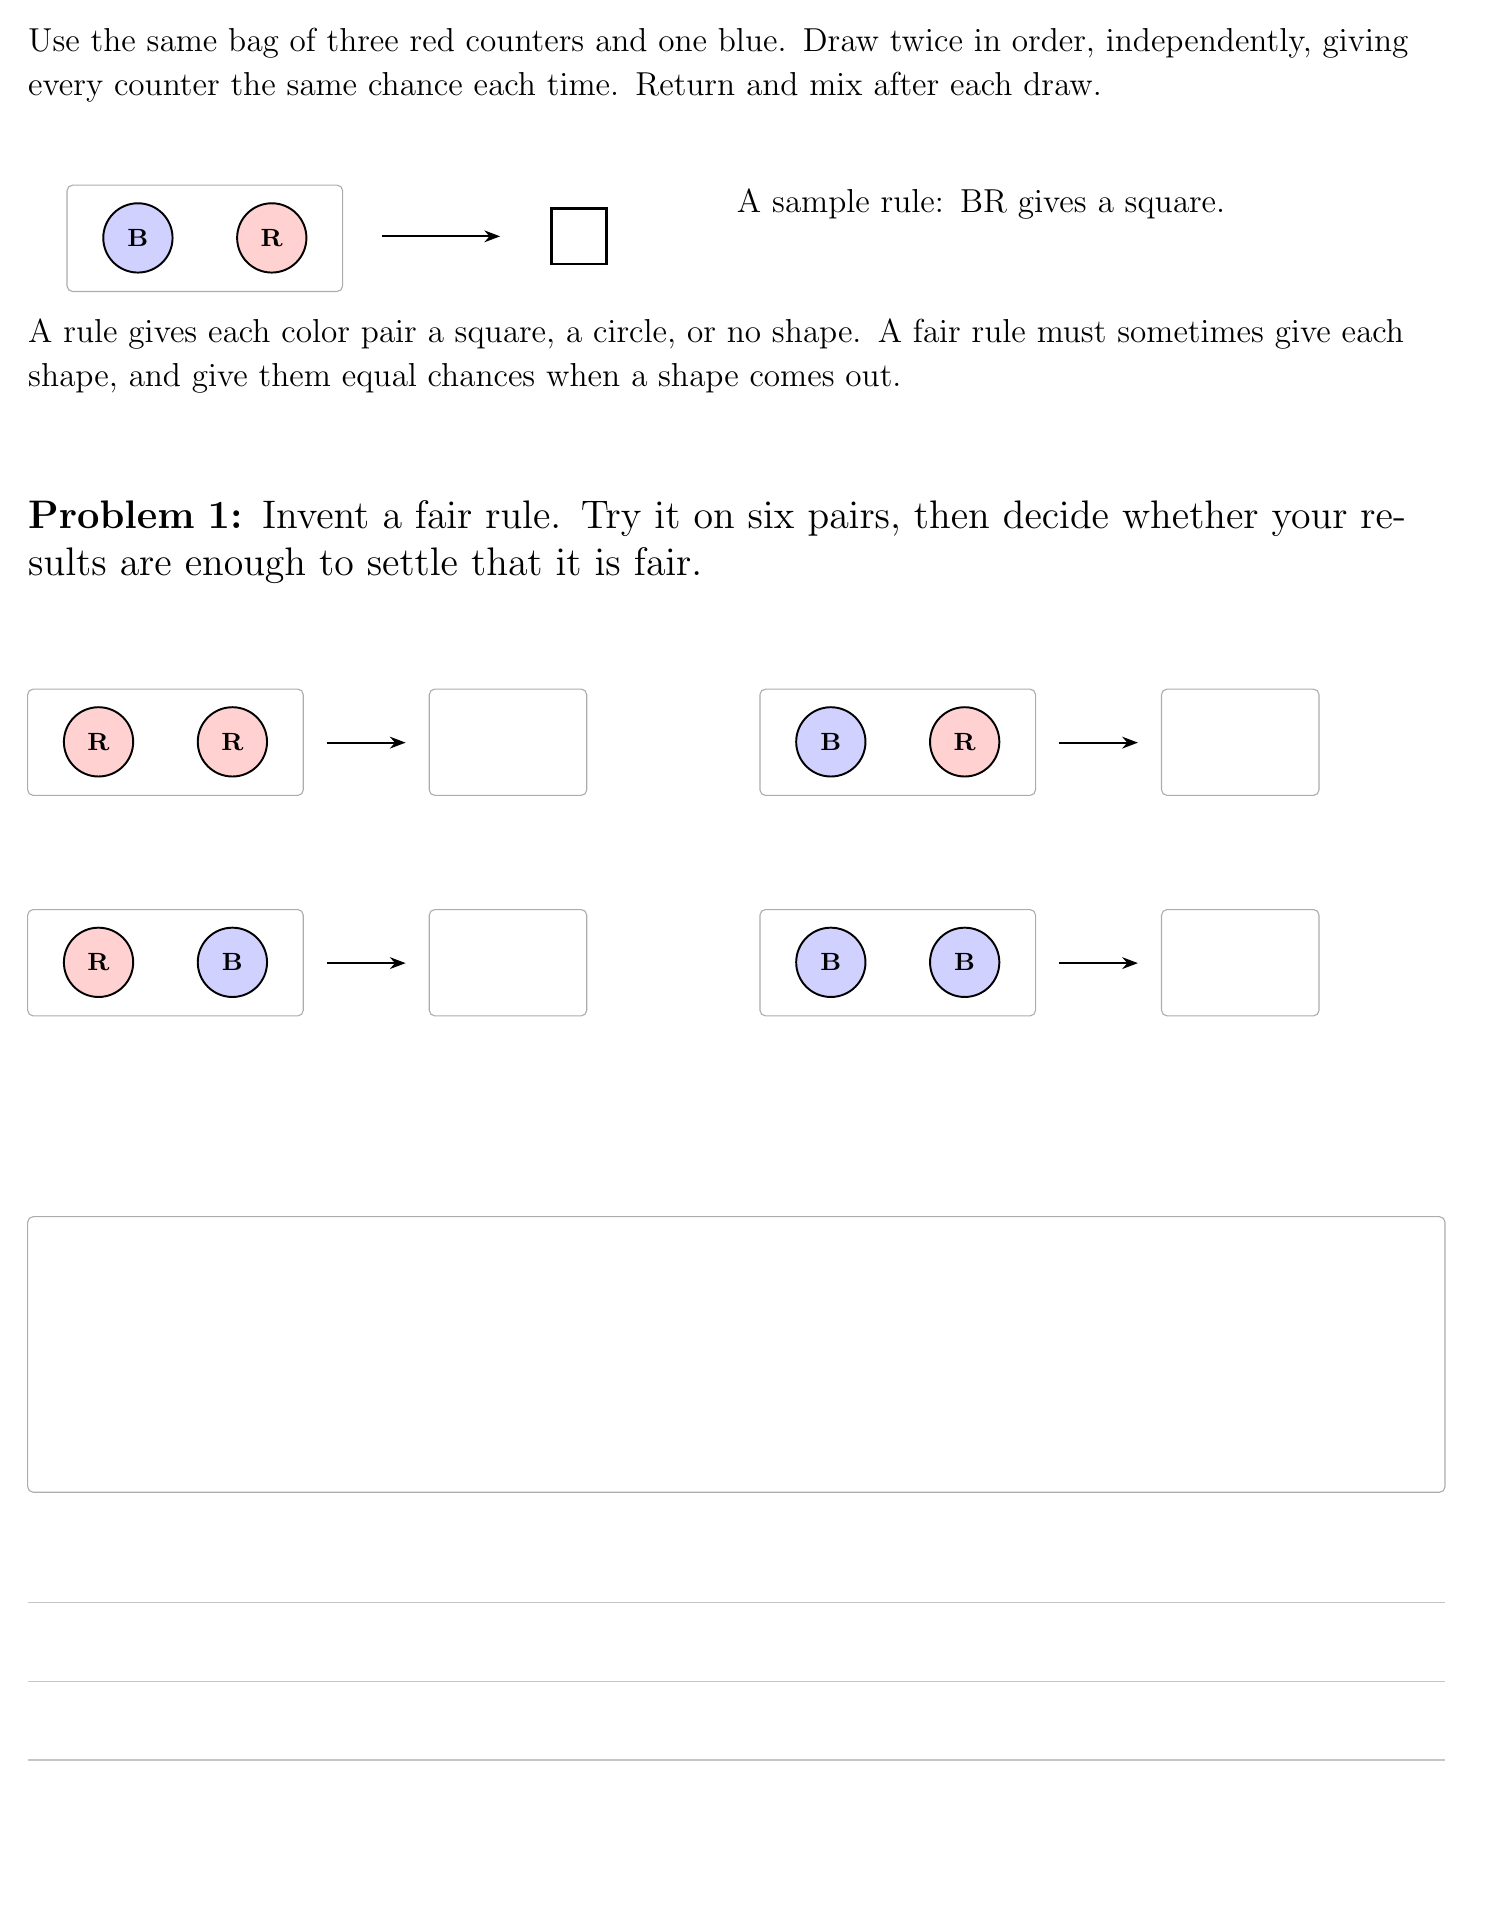
\begin{tikzpicture}[x=1cm,y=1cm]\path[use as bounding box] (0,0) rectangle (18.2,-23.6);
\node[anchor=north west,text width=18cm,inner sep=0pt,font=\fontsize{13}{16}\selectfont] at (0,0) {Use the same bag of three red counters and one blue. Draw twice in order, independently, giving every counter the same chance each time. Return and mix after each draw.};
\draw[gray!65,rounded corners=2pt] (0.5,-2) rectangle (4.0,-3.35);
\draw[fill=blue!18,line width=.7pt] (1.4,-2.67) circle (0.44);
\node[font=\bfseries\small] at (1.4,-2.67) {B};
\draw[fill=red!18,line width=.7pt] (3.1,-2.67) circle (0.44);
\node[font=\bfseries\small] at (3.1,-2.67) {R};
\draw[-{Stealth[length=2mm]},line width=.8pt] (4.5,-2.65) -- (6,-2.65) node[midway,above,font=\small] {};
\draw[line width=1pt] (6.65,-3.0) rectangle (7.35,-2.3);
\node[anchor=north west,text width=8.5cm,inner sep=0pt,font=\fontsize{12}{15}\selectfont] at (9,-2.05) {A sample rule: BR gives a square.};
\node[anchor=north west,text width=18cm,inner sep=0pt,font=\fontsize{13}{16}\selectfont] at (0,-3.7) {A rule gives each color pair a square, a circle, or no shape. A fair rule must sometimes give each shape, and give them equal chances when a shape comes out.};
\node[anchor=north west,text width=18cm,inner sep=0pt,font=\fontsize{14}{17}\selectfont] at (0,-6) {\textbf{Problem 1:} Invent a fair rule. Try it on six pairs, then decide whether your results are enough to settle that it is fair.};
\draw[gray!65,rounded corners=2pt] (0,-8.4) rectangle (3.5,-9.75);
\draw[fill=red!18,line width=.7pt] (0.9,-9.07) circle (0.44);
\node[font=\bfseries\small] at (0.9,-9.07) {R};
\draw[fill=red!18,line width=.7pt] (2.6,-9.07) circle (0.44);
\node[font=\bfseries\small] at (2.6,-9.07) {R};
\draw[-{Stealth[length=2mm]},line width=.8pt] (3.8,-9.08) -- (4.8,-9.08) node[midway,above,font=\small] {};
\draw[gray!65,rounded corners=2pt] (5.1,-8.4) rectangle (7.1,-9.75);
\draw[gray!65,rounded corners=2pt] (0,-11.2) rectangle (3.5,-12.549999999999999);
\draw[fill=red!18,line width=.7pt] (0.9,-11.87) circle (0.44);
\node[font=\bfseries\small] at (0.9,-11.87) {R};
\draw[fill=blue!18,line width=.7pt] (2.6,-11.87) circle (0.44);
\node[font=\bfseries\small] at (2.6,-11.87) {B};
\draw[-{Stealth[length=2mm]},line width=.8pt] (3.8,-11.879999999999999) -- (4.8,-11.879999999999999) node[midway,above,font=\small] {};
\draw[gray!65,rounded corners=2pt] (5.1,-11.2) rectangle (7.1,-12.549999999999999);
\draw[gray!65,rounded corners=2pt] (9.3,-8.4) rectangle (12.8,-9.75);
\draw[fill=blue!18,line width=.7pt] (10.200000000000001,-9.07) circle (0.44);
\node[font=\bfseries\small] at (10.200000000000001,-9.07) {B};
\draw[fill=red!18,line width=.7pt] (11.9,-9.07) circle (0.44);
\node[font=\bfseries\small] at (11.9,-9.07) {R};
\draw[-{Stealth[length=2mm]},line width=.8pt] (13.100000000000001,-9.08) -- (14.100000000000001,-9.08) node[midway,above,font=\small] {};
\draw[gray!65,rounded corners=2pt] (14.4,-8.4) rectangle (16.4,-9.75);
\draw[gray!65,rounded corners=2pt] (9.3,-11.2) rectangle (12.8,-12.549999999999999);
\draw[fill=blue!18,line width=.7pt] (10.200000000000001,-11.87) circle (0.44);
\node[font=\bfseries\small] at (10.200000000000001,-11.87) {B};
\draw[fill=blue!18,line width=.7pt] (11.9,-11.87) circle (0.44);
\node[font=\bfseries\small] at (11.9,-11.87) {B};
\draw[-{Stealth[length=2mm]},line width=.8pt] (13.100000000000001,-11.879999999999999) -- (14.100000000000001,-11.879999999999999) node[midway,above,font=\small] {};
\draw[gray!65,rounded corners=2pt] (14.4,-11.2) rectangle (16.4,-12.549999999999999);
\draw[gray!65,rounded corners=2pt] (0,-15.1) rectangle (18,-18.6);
\draw[gray!45] (0,-20) -- (18,-20);
\draw[gray!45] (0,-21) -- (18,-21);
\draw[gray!45] (0,-22) -- (18,-22);
\end{tikzpicture}
\newpage
\noindent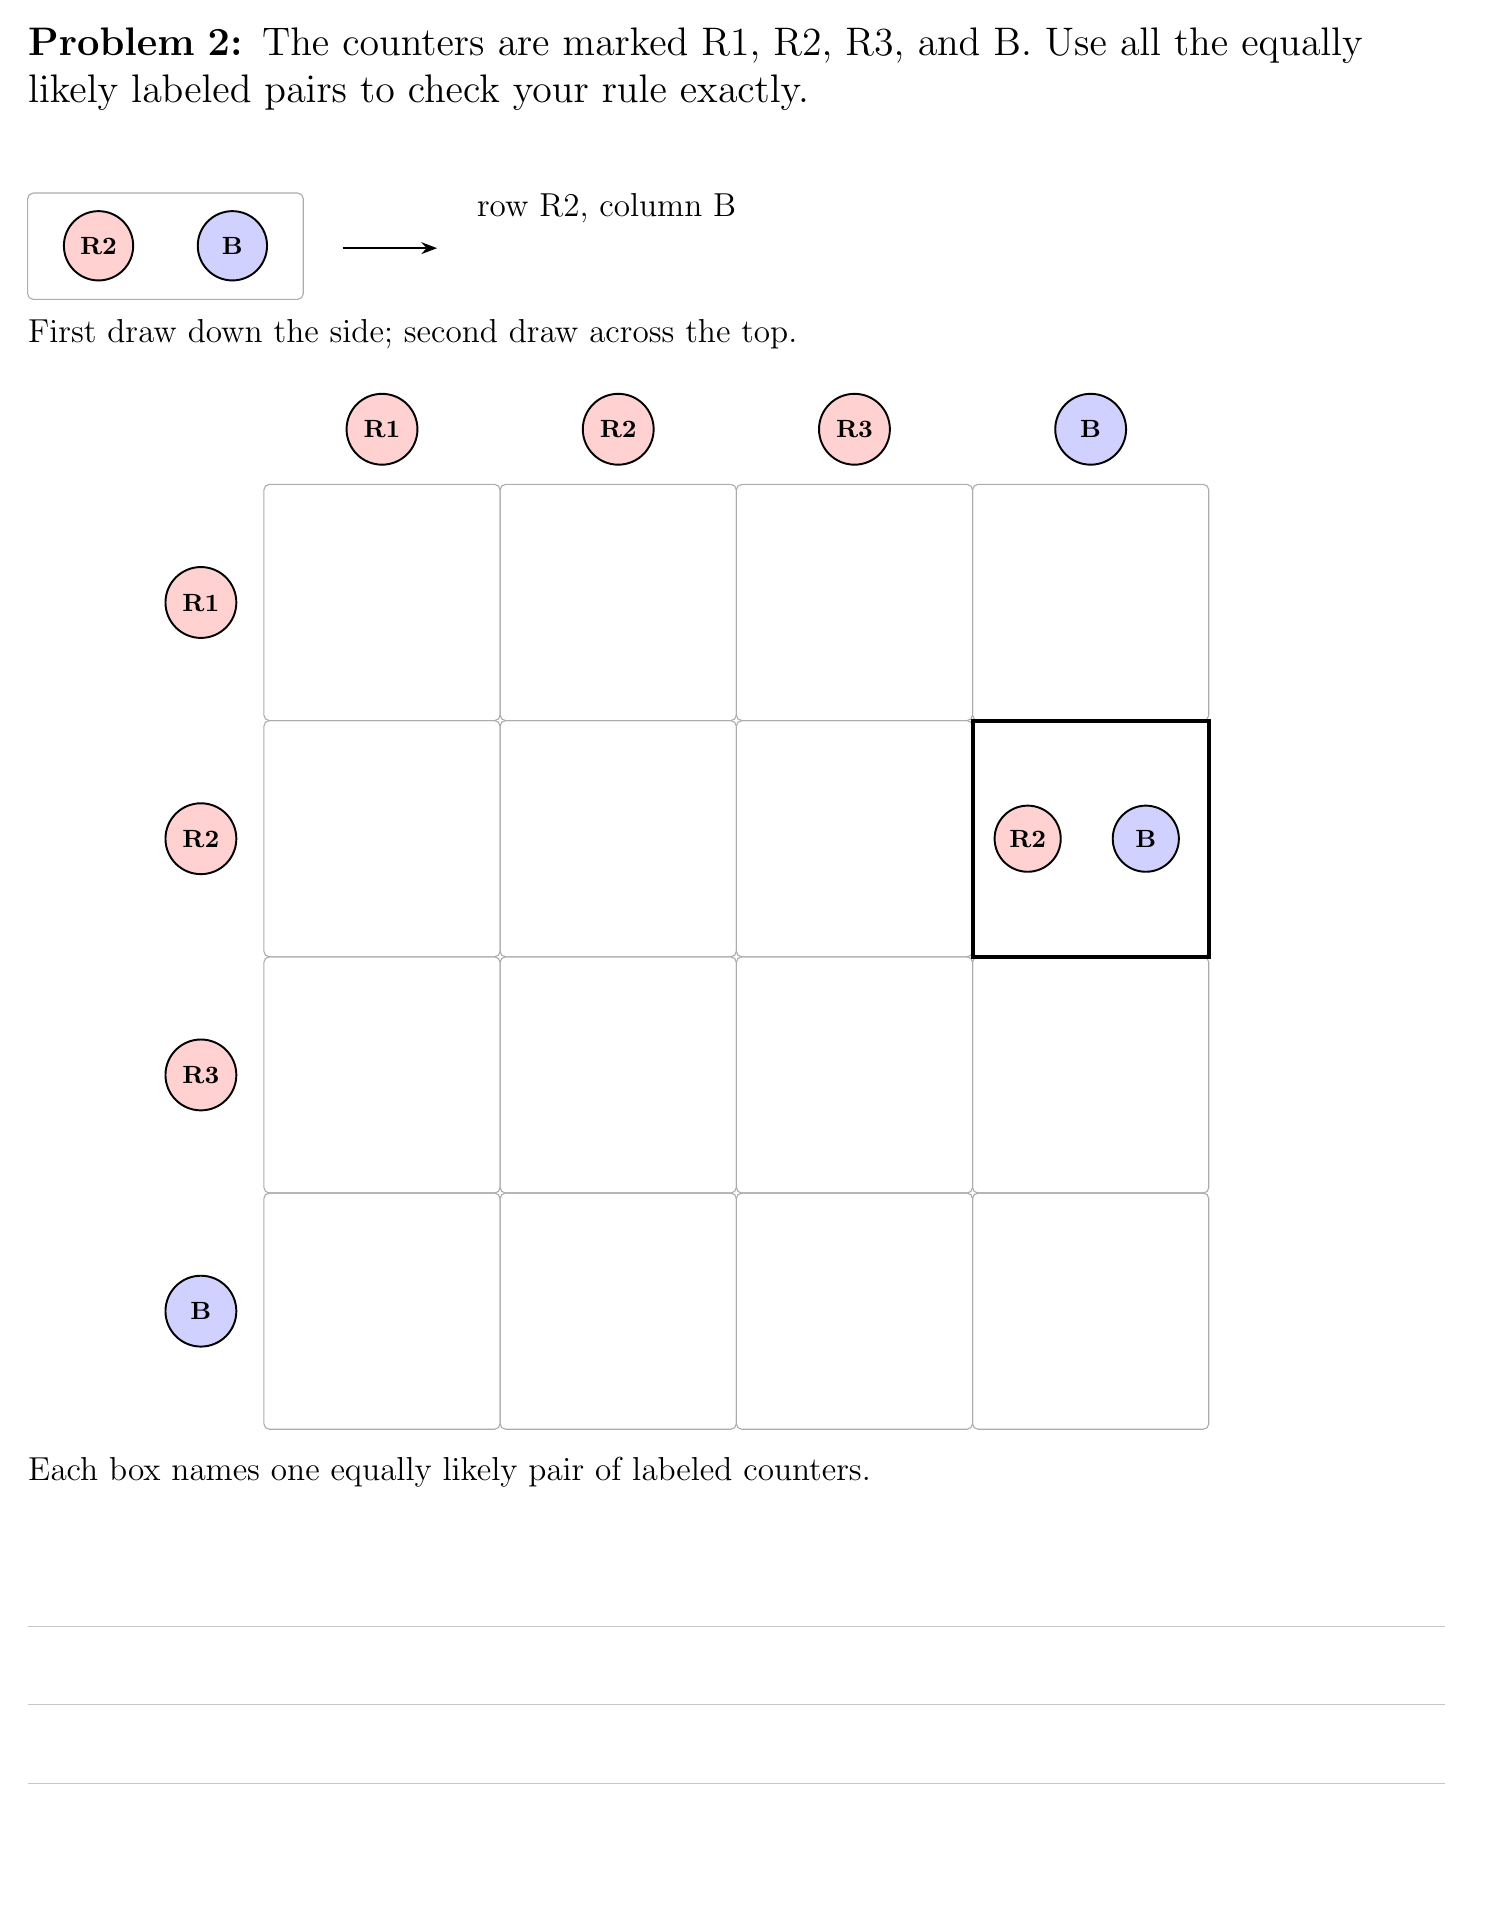
\begin{tikzpicture}[x=1cm,y=1cm]\path[use as bounding box] (0,0) rectangle (18.2,-23.6);
\node[anchor=north west,text width=18cm,inner sep=0pt,font=\fontsize{14}{17}\selectfont] at (0,0) {\textbf{Problem 2:} The counters are marked R1, R2, R3, and B. Use all the equally likely labeled pairs to check your rule exactly.};
\draw[gray!65,rounded corners=2pt] (0,-2.1) rectangle (3.5,-3.45);
\draw[fill=red!18,line width=.7pt] (0.9,-2.77) circle (0.44);
\node[font=\bfseries\small] at (0.9,-2.77) {R2};
\draw[fill=blue!18,line width=.7pt] (2.6,-2.77) circle (0.44);
\node[font=\bfseries\small] at (2.6,-2.77) {B};
\draw[-{Stealth[length=2mm]},line width=.8pt] (4,-2.8) -- (5.2,-2.8) node[midway,above,font=\small] {};
\node[anchor=north west,text width=10cm,inner sep=0pt,font=\fontsize{13}{16}\selectfont] at (5.7,-2.1) {row R2, column B};
\node[anchor=north west,text width=18cm,inner sep=0pt,font=\fontsize{12}{15}\selectfont] at (0,-3.6999999999999997) {First draw down the side; second draw across the top.};
\draw[fill=red!18,line width=.7pt] (4.5,-5.1) circle (0.45);
\node[font=\bfseries\small] at (4.5,-5.1) {R1};
\draw[fill=red!18,line width=.7pt] (2.2,-7.3) circle (0.45);
\node[font=\bfseries\small] at (2.2,-7.3) {R1};
\draw[gray!65,rounded corners=2pt] (3,-5.8) rectangle (6,-8.8);
\draw[gray!65,rounded corners=2pt] (6,-5.8) rectangle (9,-8.8);
\draw[gray!65,rounded corners=2pt] (9,-5.8) rectangle (12,-8.8);
\draw[gray!65,rounded corners=2pt] (12,-5.8) rectangle (15,-8.8);
\draw[fill=red!18,line width=.7pt] (7.5,-5.1) circle (0.45);
\node[font=\bfseries\small] at (7.5,-5.1) {R2};
\draw[fill=red!18,line width=.7pt] (2.2,-10.3) circle (0.45);
\node[font=\bfseries\small] at (2.2,-10.3) {R2};
\draw[gray!65,rounded corners=2pt] (3,-8.8) rectangle (6,-11.8);
\draw[gray!65,rounded corners=2pt] (6,-8.8) rectangle (9,-11.8);
\draw[gray!65,rounded corners=2pt] (9,-8.8) rectangle (12,-11.8);
\draw[gray!65,rounded corners=2pt] (12,-8.8) rectangle (15,-11.8);
\draw[fill=red!18,line width=.7pt] (10.5,-5.1) circle (0.45);
\node[font=\bfseries\small] at (10.5,-5.1) {R3};
\draw[fill=red!18,line width=.7pt] (2.2,-13.3) circle (0.45);
\node[font=\bfseries\small] at (2.2,-13.3) {R3};
\draw[gray!65,rounded corners=2pt] (3,-11.8) rectangle (6,-14.8);
\draw[gray!65,rounded corners=2pt] (6,-11.8) rectangle (9,-14.8);
\draw[gray!65,rounded corners=2pt] (9,-11.8) rectangle (12,-14.8);
\draw[gray!65,rounded corners=2pt] (12,-11.8) rectangle (15,-14.8);
\draw[fill=blue!18,line width=.7pt] (13.5,-5.1) circle (0.45);
\node[font=\bfseries\small] at (13.5,-5.1) {B};
\draw[fill=blue!18,line width=.7pt] (2.2,-16.3) circle (0.45);
\node[font=\bfseries\small] at (2.2,-16.3) {B};
\draw[gray!65,rounded corners=2pt] (3,-14.8) rectangle (6,-17.8);
\draw[gray!65,rounded corners=2pt] (6,-14.8) rectangle (9,-17.8);
\draw[gray!65,rounded corners=2pt] (9,-14.8) rectangle (12,-17.8);
\draw[gray!65,rounded corners=2pt] (12,-14.8) rectangle (15,-17.8);
\draw[line width=1.4pt] (12,-8.8) rectangle (15,-11.8);
\draw[fill=red!18,line width=.7pt] (12.7,-10.3) circle (0.42);
\node[font=\bfseries\small] at (12.7,-10.3) {R2};
\draw[fill=blue!18,line width=.7pt] (14.2,-10.3) circle (0.42);
\node[font=\bfseries\small] at (14.2,-10.3) {B};
\node[anchor=north west,text width=18cm,inner sep=0pt,font=\fontsize{12}{15}\selectfont] at (0,-18.15) {Each box names one equally likely pair of labeled counters.};
\draw[gray!45] (0,-20.3) -- (18,-20.3);
\draw[gray!45] (0,-21.3) -- (18,-21.3);
\draw[gray!45] (0,-22.3) -- (18,-22.3);
\end{tikzpicture}
\newpage
\noindent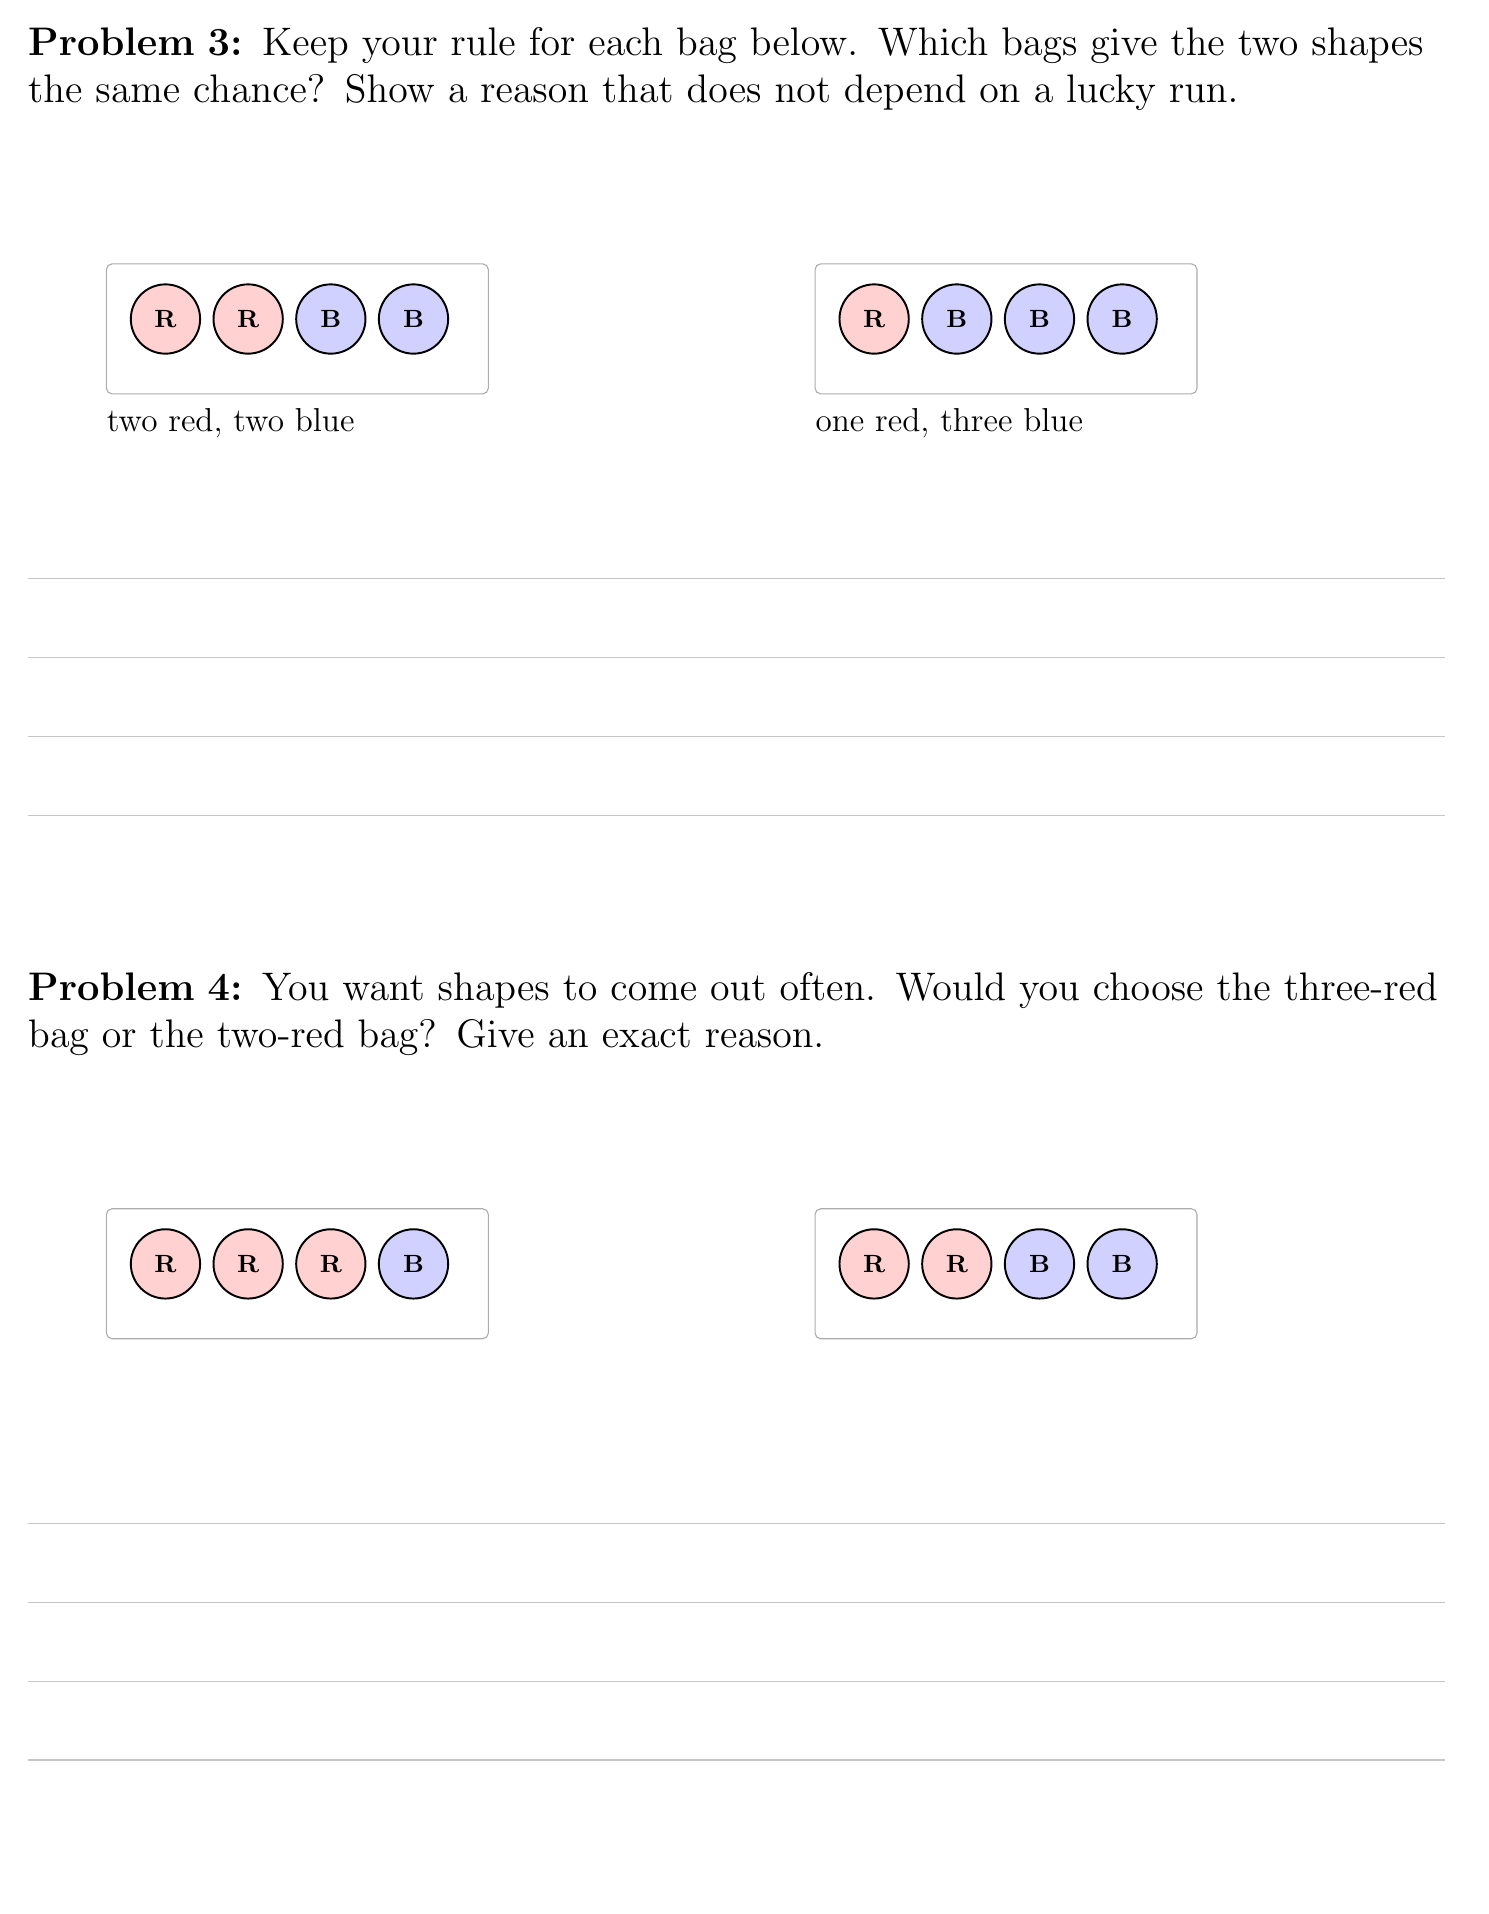
\begin{tikzpicture}[x=1cm,y=1cm]\path[use as bounding box] (0,0) rectangle (18.2,-23.6);
\node[anchor=north west,text width=18cm,inner sep=0pt,font=\fontsize{14}{17}\selectfont] at (0,0) {\textbf{Problem 3:} Keep your rule for each bag below. Which bags give the two shapes the same chance? Show a reason that does not depend on a lucky run.};
\draw[gray!65,rounded corners=2pt] (1,-3) rectangle (5.8500000000000005,-4.65);
\draw[fill=red!18,line width=.7pt] (1.75,-3.7) circle (0.44);
\node[font=\bfseries\small] at (1.75,-3.7) {R};
\draw[fill=red!18,line width=.7pt] (2.8,-3.7) circle (0.44);
\node[font=\bfseries\small] at (2.8,-3.7) {R};
\draw[fill=blue!18,line width=.7pt] (3.85,-3.7) circle (0.44);
\node[font=\bfseries\small] at (3.85,-3.7) {B};
\draw[fill=blue!18,line width=.7pt] (4.9,-3.7) circle (0.44);
\node[font=\bfseries\small] at (4.9,-3.7) {B};
\node[anchor=north west,text width=4.8500000000000005cm,inner sep=0pt,font=\fontsize{12}{15}\selectfont] at (1,-4.83) {two red, two blue};
\draw[gray!65,rounded corners=2pt] (10,-3) rectangle (14.850000000000001,-4.65);
\draw[fill=red!18,line width=.7pt] (10.75,-3.7) circle (0.44);
\node[font=\bfseries\small] at (10.75,-3.7) {R};
\draw[fill=blue!18,line width=.7pt] (11.8,-3.7) circle (0.44);
\node[font=\bfseries\small] at (11.8,-3.7) {B};
\draw[fill=blue!18,line width=.7pt] (12.85,-3.7) circle (0.44);
\node[font=\bfseries\small] at (12.85,-3.7) {B};
\draw[fill=blue!18,line width=.7pt] (13.9,-3.7) circle (0.44);
\node[font=\bfseries\small] at (13.9,-3.7) {B};
\node[anchor=north west,text width=4.8500000000000005cm,inner sep=0pt,font=\fontsize{12}{15}\selectfont] at (10,-4.83) {one red, three blue};
\draw[gray!45] (0,-7) -- (18,-7);
\draw[gray!45] (0,-8) -- (18,-8);
\draw[gray!45] (0,-9) -- (18,-9);
\draw[gray!45] (0,-10) -- (18,-10);
\node[anchor=north west,text width=18cm,inner sep=0pt,font=\fontsize{14}{17}\selectfont] at (0,-12) {\textbf{Problem 4:} You want shapes to come out often. Would you choose the three-red bag or the two-red bag? Give an exact reason.};
\draw[gray!65,rounded corners=2pt] (1,-15) rectangle (5.8500000000000005,-16.65);
\draw[fill=red!18,line width=.7pt] (1.75,-15.7) circle (0.44);
\node[font=\bfseries\small] at (1.75,-15.7) {R};
\draw[fill=red!18,line width=.7pt] (2.8,-15.7) circle (0.44);
\node[font=\bfseries\small] at (2.8,-15.7) {R};
\draw[fill=red!18,line width=.7pt] (3.85,-15.7) circle (0.44);
\node[font=\bfseries\small] at (3.85,-15.7) {R};
\draw[fill=blue!18,line width=.7pt] (4.9,-15.7) circle (0.44);
\node[font=\bfseries\small] at (4.9,-15.7) {B};
\draw[gray!65,rounded corners=2pt] (10,-15) rectangle (14.850000000000001,-16.65);
\draw[fill=red!18,line width=.7pt] (10.75,-15.7) circle (0.44);
\node[font=\bfseries\small] at (10.75,-15.7) {R};
\draw[fill=red!18,line width=.7pt] (11.8,-15.7) circle (0.44);
\node[font=\bfseries\small] at (11.8,-15.7) {R};
\draw[fill=blue!18,line width=.7pt] (12.85,-15.7) circle (0.44);
\node[font=\bfseries\small] at (12.85,-15.7) {B};
\draw[fill=blue!18,line width=.7pt] (13.9,-15.7) circle (0.44);
\node[font=\bfseries\small] at (13.9,-15.7) {B};
\draw[gray!45] (0,-19) -- (18,-19);
\draw[gray!45] (0,-20) -- (18,-20);
\draw[gray!45] (0,-21) -- (18,-21);
\draw[gray!45] (0,-22) -- (18,-22);
\end{tikzpicture}
\newpage
\noindent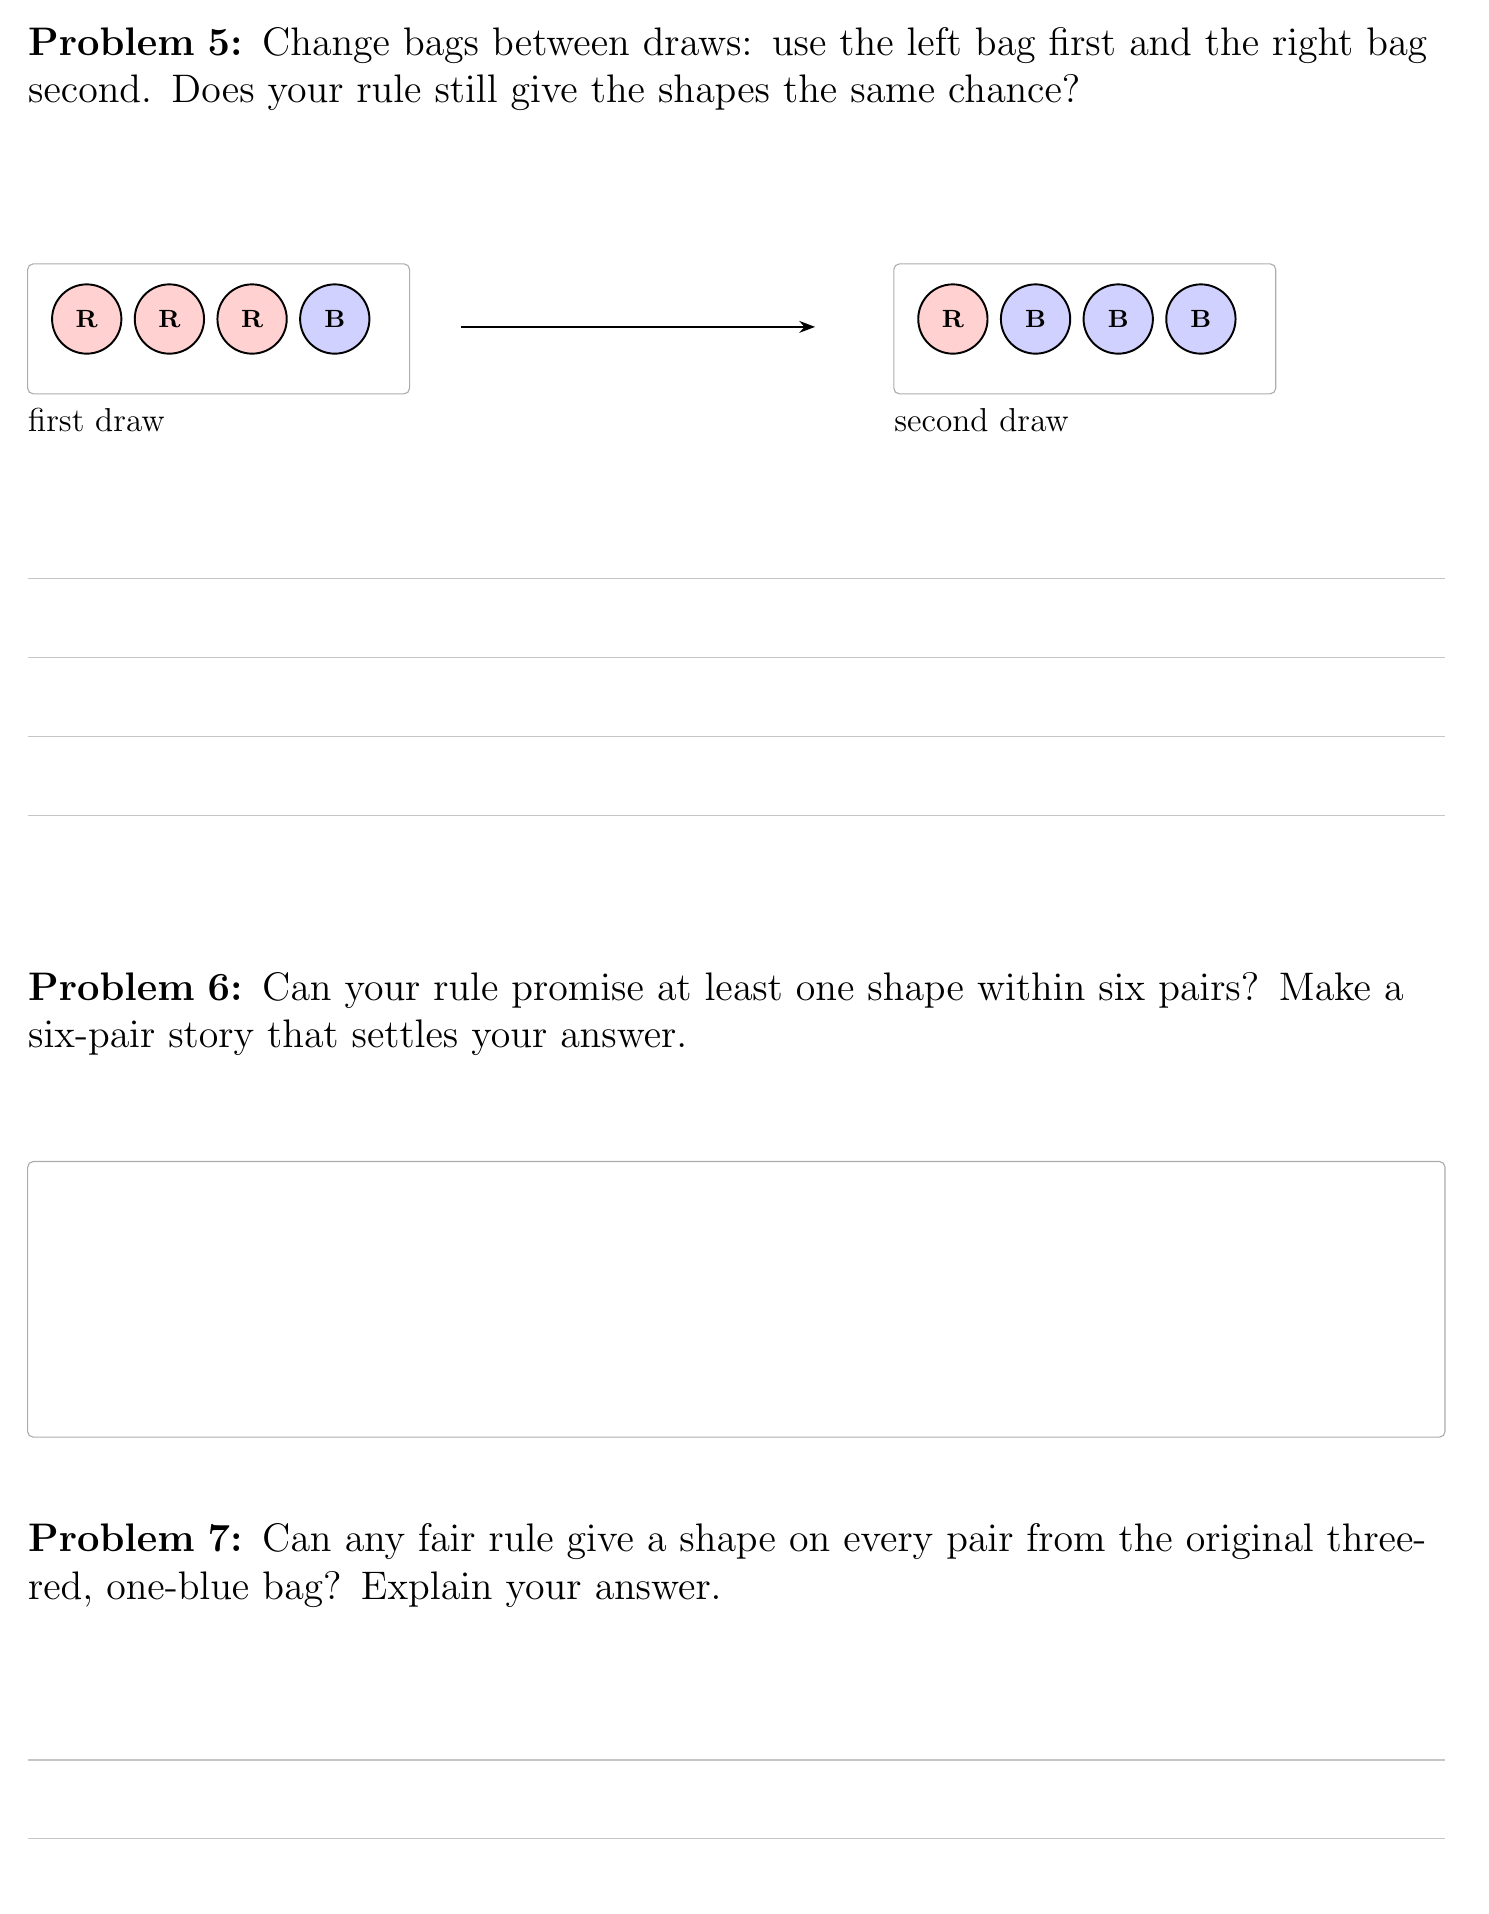
\begin{tikzpicture}[x=1cm,y=1cm]\path[use as bounding box] (0,0) rectangle (18.2,-23.6);
\node[anchor=north west,text width=18cm,inner sep=0pt,font=\fontsize{14}{17}\selectfont] at (0,0) {\textbf{Problem 5:} Change bags between draws: use the left bag first and the right bag second. Does your rule still give the shapes the same chance?};
\draw[gray!65,rounded corners=2pt] (0,-3) rectangle (4.8500000000000005,-4.65);
\draw[fill=red!18,line width=.7pt] (0.75,-3.7) circle (0.44);
\node[font=\bfseries\small] at (0.75,-3.7) {R};
\draw[fill=red!18,line width=.7pt] (1.8,-3.7) circle (0.44);
\node[font=\bfseries\small] at (1.8,-3.7) {R};
\draw[fill=red!18,line width=.7pt] (2.85,-3.7) circle (0.44);
\node[font=\bfseries\small] at (2.85,-3.7) {R};
\draw[fill=blue!18,line width=.7pt] (3.9000000000000004,-3.7) circle (0.44);
\node[font=\bfseries\small] at (3.9000000000000004,-3.7) {B};
\node[anchor=north west,text width=4.8500000000000005cm,inner sep=0pt,font=\fontsize{12}{15}\selectfont] at (0,-4.83) {first draw};
\draw[gray!65,rounded corners=2pt] (11,-3) rectangle (15.850000000000001,-4.65);
\draw[fill=red!18,line width=.7pt] (11.75,-3.7) circle (0.44);
\node[font=\bfseries\small] at (11.75,-3.7) {R};
\draw[fill=blue!18,line width=.7pt] (12.8,-3.7) circle (0.44);
\node[font=\bfseries\small] at (12.8,-3.7) {B};
\draw[fill=blue!18,line width=.7pt] (13.85,-3.7) circle (0.44);
\node[font=\bfseries\small] at (13.85,-3.7) {B};
\draw[fill=blue!18,line width=.7pt] (14.9,-3.7) circle (0.44);
\node[font=\bfseries\small] at (14.9,-3.7) {B};
\node[anchor=north west,text width=4.8500000000000005cm,inner sep=0pt,font=\fontsize{12}{15}\selectfont] at (11,-4.83) {second draw};
\draw[-{Stealth[length=2mm]},line width=.8pt] (5.5,-3.8) -- (10,-3.8) node[midway,above,font=\small] {};
\draw[gray!45] (0,-7) -- (18,-7);
\draw[gray!45] (0,-8) -- (18,-8);
\draw[gray!45] (0,-9) -- (18,-9);
\draw[gray!45] (0,-10) -- (18,-10);
\node[anchor=north west,text width=18cm,inner sep=0pt,font=\fontsize{14}{17}\selectfont] at (0,-12) {\textbf{Problem 6:} Can your rule promise at least one shape within six pairs? Make a six-pair story that settles your answer.};
\draw[gray!65,rounded corners=2pt] (0,-14.4) rectangle (18,-17.9);
\node[anchor=north west,text width=18cm,inner sep=0pt,font=\fontsize{14}{17}\selectfont] at (0,-19) {\textbf{Problem 7:} Can any fair rule give a shape on every pair from the original three-red, one-blue bag? Explain your answer.};
\draw[gray!45] (0,-22) -- (18,-22);
\draw[gray!45] (0,-23) -- (18,-23);
\end{tikzpicture}
\end{document}
